\documentclass{article}
\usepackage{graphicx} % Required for inserting images

\title{DevOps, Software Evolution and Software Maintenance\\
\large Course Code: BSDSESM1KU}
\author{GitGurus - Group K}
\date{May 23, 2024}

% \usepackage{graphicx} % Required for inserting images
% \usepackage{amsmath}
% \usepackage{hyperref}
\usepackage{listings}
\lstset
{
    basicstyle=\footnotesize,
    numbers=left,
    stepnumber=1,
    showstringspaces=false,
    tabsize=1,
    breaklines=true,
    breakatwhitespace=false,
}

\usepackage[utf8]{inputenc}
\usepackage[T1]{fontenc}
\usepackage[english]{babel}
\usepackage{minted}
% \usepackage[a4paper, bottom=3cm, top=3cm, left=2.5cm, right=2.5cm]{geometry}
\usepackage[linewidth=1pt]{mdframed}
\usepackage{ebproof}
\usepackage{amsmath}
% \usepackage{fourier}
\usepackage{booktabs}
% \usepackage{inconsolata}
\usepackage{float}
\usepackage{lastpage}
\usepackage{graphicx}
\usepackage{titling}
\usepackage{fancyhdr}
\usepackage[dvipsnames]{xcolor}
\usepackage[hidelinks]{hyperref}

\renewcommand{\baselinestretch}{1.2} % Line spacing
% \setlength{\parindent}{0em} % Paragraph indent
% \setlength{\parskip}{0.75em} % Paragraph vertical spacing

% \colorlet{LightGray}{Gray!7!}

% % global minted styles
% \setminted{bgcolor=LightGray, breaklines, frame=single, linenos, fontsize=\small, numbersep=8pt}

% % minted remove red squares around "erroneus" code
% \AtBeginEnvironment{minted}{%
%   \renewcommand{\fcolorbox}[4][]{#4}}

% % minted line number style
% \renewcommand{\theFancyVerbLine}{{\scriptsize \arabic{FancyVerbLine}}}
\begin{document}

\maketitle
\thispagestyle{empty}
\setcounter{page}{0}
\vspace{2cm}

\begin{table}[H]
    \centering
    \begin{tabular}{r|l}
    Andreas Guldborg Hansen & aguh@itu \\
    Andreas Severin Hauch Trøstrup & atro@itu.dk \\
    Frederik Petersen & frepe@itu.dk \\
    Mads Aqqalu Roager & mroa@itu.dk \\
    Silke Sofie Holme Bonnén & ssbo@itu.dk
    \end{tabular}
\end{table}

\newpage
\tableofcontents

\newpage


\section{Systems' perspective}
\subsection{Design and architecture}
An overview of the architecture of our MiniTwit application can be found in Figure \ref{fig:architecture}. 
The entire system operates on DigitalOcean, except for our monitoring and logging functions, which are managed through New Relic. In DigitalOcean, we have three primary nodes. A swarm manager, and two workers. These 3 nodes are a part of a Docker swarm network that runs the MiniTwit web app and MiniTwit simulator API containers as Docker services.
The workers and manager also run a New Relic agent that collects logs and system monitoring metrics. This information is then sent to New Relic.
The manager node runs an Nginx reverse proxy, that serves a certificate to allow for SSL encryption, and load balances between the workers and the manager.
Lastly, the database for our application is managed by DigitalOcean.

\begin{figure}[H]
    \centering
    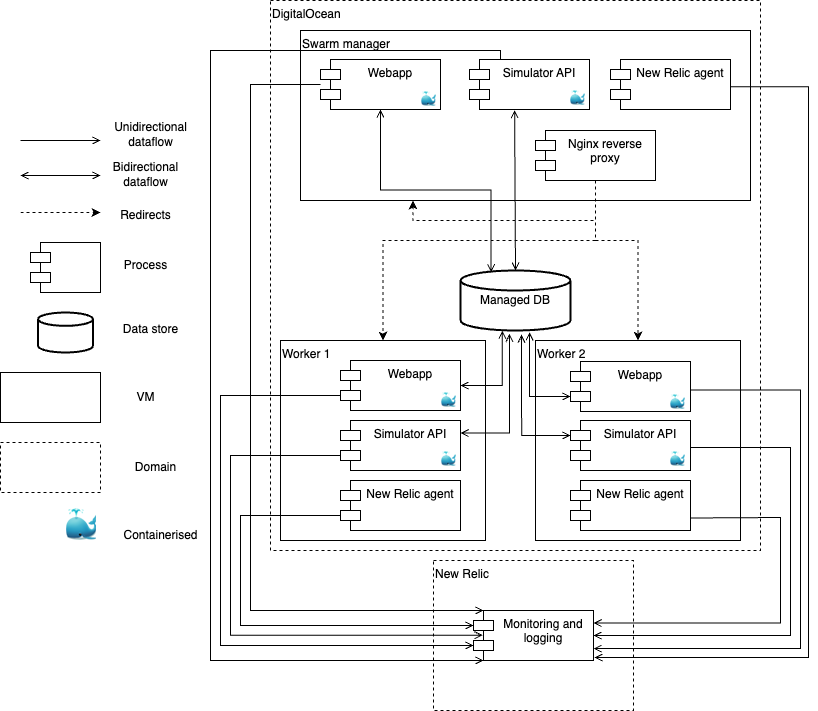
\includegraphics[width=\textwidth]{images/devops-overview-3.png}
    \caption{The figure shows a diagram of the architecture of MiniTwit}
    \label{fig:architecture}
\end{figure}

\subsection{Dependencies}
Our application has numerous dependencies, so we have decided to only describe those that are critical to our application in production. That is, if there is a problem with one of these dependencies, e.g. a dependency has a open security problem, we have a problem. 

Figure \ref{fig:dep-prod} displays the production dependency graph, illustrating only direct dependencies, with the exception of PostgreSQL as a dependency of DigitalOcean due to its significance for our application. Transitive dependencies and development dependencies are not shown in Figure \ref{fig:dep-prod}. Key development dependencies are displayed in Appendix \ref{appendix: dev-dependecies}.

\begin{figure}[H]
    \centering
    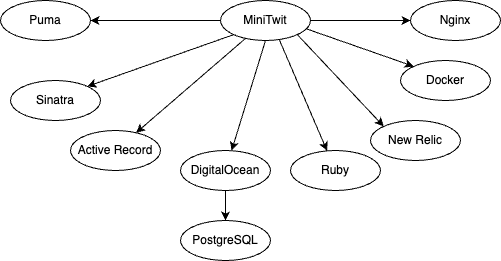
\includegraphics[width=0.8\textwidth]{images/dependency-graph-prod.png}
    \caption{Production dependency graph.}
    \label{fig:dep-prod}
\end{figure}

Puma is the web server used for serving requests to our Ruby application. 
To develop our web application we use Sinatra, which is a web application library for Ruby. 
The Object-Relational Mapping (ORM) library ``Active Record'' is used to simplify interactions with the database. This enables us to avoid having SQL statements in our code which keeps the code more clean and reduces the possibility of SQL injections from improperly escaped SQL statements.
DigitalOcean is the only critical dependency for keeping the application running, as this is where our PostgreSQL database server and virtual machines are hosted.
Ruby is the programming language used to develop the MiniTwit application.
New Relic is used for monitoring and logging of the system. 
Docker is used for containerization of our application, such that it can run anywhere Docker is installed. The application is run with Docker Swarm, which ensures that the application runs across several machines, and makes load-balancing possible. It also makes it possible to make updates to the application with minimal downtime.
Nginx is a reverse proxy and load balancer we use to redirect HTTP requests from minitwit.tech to our replicated MiniTwit application. 
It takes the reply from the worker and replies the client through https://minitwit.tech with a certificate signed by LetsEncrypt, 
and thus achieves both load balancing and security in the form of SSL encryption.

\subsection{Interactions of subsystems}

The interactions between MiniTwit's subsystems is explained through two sequence diagrams of a user interacting with MiniTwit's web app and the API. 

Diagram \ref{fig:sequence} starts with a user trying to access minitwit.tech through a browser. The first part of the diagram shows how the DNS protocol is utilized in order to get the IP address of the server. The second part shows how the Nginx reverse proxy, located inside the swarm manager, forwards the HTTP request to worker 1 or 2. Inside the worker the web application is running in a container. When the application gets the request it queries the database to get the latest messages. While the application handles the request a New Relic Ruby agent monitors the request and forwards application performance metrics to New Relic. Finally a response gets propagated all the way back to the browser.

Similarly, the diagram for the simulator API available in Figure \ref{fig:sequence_api} starts with the actor sending a HTTP GET request to api.minitwit.tech/msgs. In this diagram we omitted the DNS protocol as it is shown in detail in Figure \ref{fig:sequence}. The Nginx reverse proxy forwards the request to worker 1 or 2, that then checks if the request originated from the simulator by checking if the header of the request was set correctly. If it was, it queries the database for the latest \texttt{no} messages, where \texttt{no} denotes a parameter set to specify how many messages should be returned. Like in Figure \ref{fig:sequence}, we handle logging and monitoring before propagating the response.

\begin{figure}[H]
    \centering
    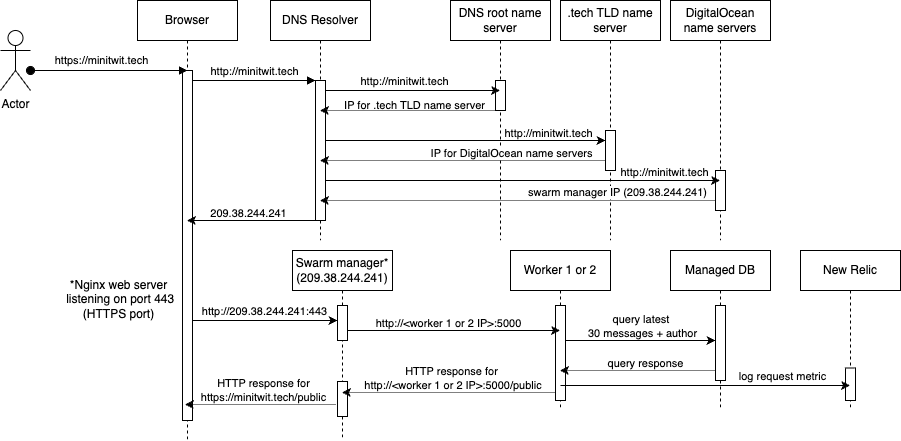
\includegraphics[width=\textwidth]{images/devops-sequence.png}
    \caption{The figure shows a sequence diagram describing a HTTP GET request to "minitwit.tech". }
    \label{fig:sequence}
\end{figure}


\begin{figure}[H]
    \centering
    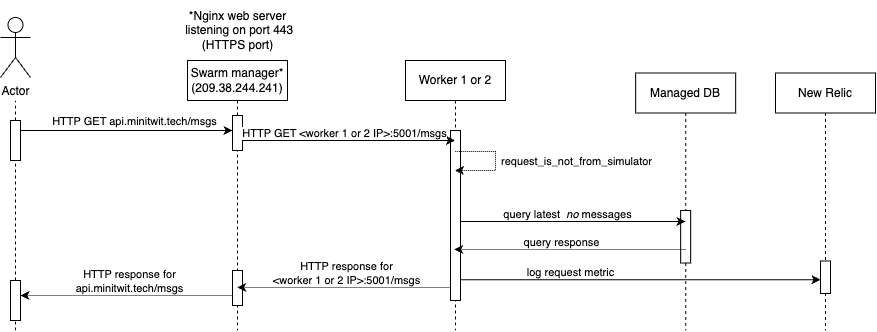
\includegraphics[width=\textwidth]{images/api-sequence.png}
    \caption{The figure shows a sequence diagram describing a HTTP GET request to "api.minitwit.tech/msgs". Since the actor is the simulator, \texttt{request\_is\_not\_from\_simulator} returns false. Otherwise it would return immediately with status code 403.}
    \label{fig:sequence_api}
\end{figure}


\subsection{Current state}
SonarCloud and CodeClimate has been used for static analysis and quality assessment. 
The quality gate status on SonarCloud is passed and there are no issues and no security hotspots detected. The duplication of code is 1.7\% which is below the 3\% limit. Code Climate maintainability rating is A, and there is one issue about a function being too long. 

To reduce noise in our static analysis the test files have been excluded from the static analysis to focus on the quality and maintainability in the application code as test files has different coding standards. An example of how 
the coding standards differ can be seen in the documentation for Playwright, our used end-to-end testing tool. They state that it is okay to have some duplication in your tests especially if it keeps your test clearer and easier to read and maintain\footnote{https://playwright.dev/docs/best-practices}. 


\section{Process' perspective}

\subsection{CI/CD chain}
Our CI/CD chain is mainly built using GitHub Actions but also includes local pre-commit hooks. Pre-commit hooks are employed to automatically run RuboCop and other linters, enforcing coding standards and consistency throughout the development process. 
In Github Actions we have implemented workflows to automate testing, releasing and deploying our code. Furthermore this is also where we use SonarCloud.

\subsubsection{Automatic testing}
When a pull request is opened on GitHub, the \texttt{automatic-testing} workflow is triggered. This workflow builds a Docker image with the branch code, and runs it as a container using our \texttt{docker-compose} configuration. The workflow then runs our test suite and reports if any tests fail.


\subsubsection{Deployment workflows}
When a commit is made to the main branch of our repository, our deployment workflow is triggered and deploys to production. 
This workflow checks out the code and logs in to \texttt{Docker Hub}. The workflow then builds the Docker image, tagging it \texttt{latest} and pushes the image to Docker Hub, making it easy to pull and build this production-ready Docker image. The last action of the workflow is to establish an \texttt{ssh} connection to the swarm manager from which it runs our deploy script.
Once \texttt{deploy.sh} runs on the manager node, it sets the necessary environment variables in order to connect to the managed database, log to New Relic and pull the correct image from Docker Hub before using \texttt{Docker Swarm's} command to execute a rolling deployment of the new Docker image. The \texttt{./remote\_files/docker-compose.yml} file is responsible for configuring the Docker swarm, such that there are three replicas of the API and the web application.

For a period of time during the project, we also had a staging environment which was deployed similar to production but by a manual trigger targeting a branch. This environment also tagged Docker images with the git commit's SHA-value instead of \texttt{latest}, and allowed us to test larger changes such as switching database management system.

\subsubsection{Release workflow}
A simple workflow exists to ensure automatic releases are created on GitHub every time new code is added to the main branch. This workflow simply uses the two actions \texttt{actions/checkout@v4} and \texttt{actions/create-release@v1} to create a release with a version tag and release name based on the commit's SHA-value.

\subsubsection{Report workflows}
To ensure our report in our repository is always up to date, we utilise a built-in synchronization between Overleaf and GitHub. Once changes are made that a group member wish to save, one click from within Overleaf synchronizes the contents to a separate repository in our GitHub organisation, which triggers two Github Actions workflows:
\begin{enumerate}
    \item A workflow from within this report repository that notifies our main repository of any changes made to our report repository.
    \item A workflow from within the main repository that is called by the previously mentioned workflow, which triggers a git submodule update and commits it to the repository.
\end{enumerate}

\subsection{Monitoring \& Logging}
Both monitoring and logging of this project is done using New Relic. By installing the New Relic agent on our VMs, and the New Relic gem in our Ruby application we can link it to the web interface. This is done via a push-based monitoring configuration, as all VMs push their data directly to New Relic. 

From the interface we can see Application Performance Monitoring (APM), and infrastructure monitoring -- this includes:
\begin{itemize}
    \item Web transaction time by application layer (See Figure \ref{fig:transaction-times})
    \item Throughput for the application (Requests per minute) 
    \item The slowest transactions, by average response time.
    \item Error rate of transactions
\end{itemize}
Additionally we have set New Relic up to send us alerts on   Slack, should the application suddenly have a significantly lower application throughput than usual, or if the error rate rises.
\begin{figure}[H]
    \centering
    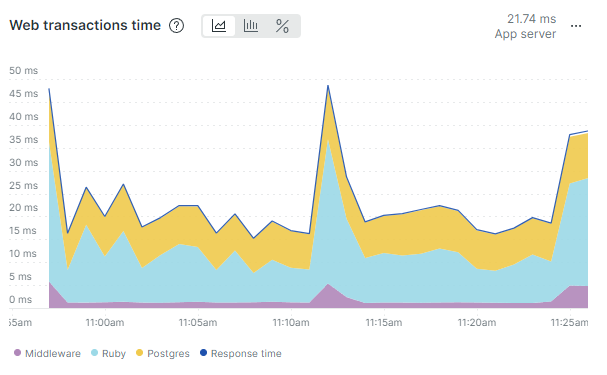
\includegraphics[width=\textwidth]{images/new-relic-transactions.png}
    \caption{The New Relic graph depicting web transaction times by application layer}
    \label{fig:transaction-times}
\end{figure}

Logs are aggregated automatically by the New Relic agent. The agent picks up log messages from any configured source. By default this includes the \texttt{linux\_syslog} and the Docker log. In our case we aggregate \texttt{linux\_auth}, \texttt{linux\_syslog} and the \texttt{nginx} logs. The nginx logs shows all request made to the application on any of the VMs.

\subsection{Security}
The results of the security assessment yielded no obvious vulnerabilities, however we have had security in mind while making the application, especially in some aspects of the system. Firstly, we use an ORM to interact with the database in the application. This means that we do not have any explicit SQL statements in the code that can be exploited, and that Active Record handles the security in terms of SQL injection prevention. Secondly, we have implemented HTTPS via. the Nginx reverse proxy. This means that all requests accessed at minitwit.tech are encrypted, and thus protects confidentiality. Lastly, we use a Docker Swarm to host the application, which makes the system more scalable and therefore easier to protect against a Distributed Denial-of-Service attack. However, certain DDoS attacks might pose a risk if they are overloading our database through large messages since the database is not replicated. This risk is somewhat mitigated by all DigitalOcean resources being DDoS protected.
We also use Dependabot such that we will get notified when any dependency has an update, or has a security vulnerability.

\subsection{Scaling and upgrading}
% NB: Vi har skrevet lidt om det her i 2.1.2. Overvej om vi skal rykke noget derfra herned eller hvordan vi klarer det.

Horizontal scaling is used as our scaling strategy. This means that whenever an upscale is necessary another node will be added to the Docker swarm as a replica of the system. We use Nginx as our load-balancer. This means that our swarm manager, which runs Nginx, becomes a single point of failure. It is always undesired to have single points of failures so if we had more time we would have liked to implement a redundant Load Balancer Setup, though this has not been investigated yet.


\subsection{Use of AI tools}
% \todo{In case you have used AI-assistants during your project briefly explain which system(s) you used during the project and reflect how it supported/hindered your process.}

In the beginning of the project, not all team members were familiar with the programming language Ruby. In order to get familiar, some of us had the Github Copilot extension enabled, allowing us to participate on a similar level as those who were more familiar with the language.
This increased productivity but may have hindered learning by providing answers directly instead of encouraging independent research.

In the review process, ChatGPT has been used as a tool to interpret changes made by other members, by prompting ChatGPT to help understand the effects and consequences of the changes. This has been a very helpful way to get complicated things explained quickly, and overall we believe that it has helped our learning experience. 

\section{Lessons learned perspective}
% \todo{Describe the biggest issues, how you solved them, and which are major lessons learned with regards to: evolution and refactoring,
% operation, and
% maintenance 
% of your ITU-MiniTwit systems. Link back to respective commit messages, issues, tickets, etc. to illustrate these. Also reflect and describe what was the "DevOps" style of your work. For example, what did you do differently to previous development projects and how did it work?}

% Paragraph: Evolving & Maintaining database (maybe)
% discuss what issues we had with migrating to new database. What did we learn from migrating
% we used New Relic to identify missing indexes, to improve query speed (maintenance)
When we started out the project, the database was running as an SQLite database on the machine which also hosted our application. As the project progressed, we decided to migrate to a managed PostgreSQL database, hosted on DigitalOcean. Migrating to this new database was one of the bigger challenges in the project, as multiple problems in the process ended up causing us downtime\footnote{\href{https://github.com/git-gurus-itu-devops/itu-minitwit/issues/25\#issuecomment-1983695933}{https://github.com/git-gurus-itu-devops/itu-minitwit/issues/25\#issuecomment-1983695933}}.
The biggest issue was in how we transferred the data from SQLite to the new database. We created a simple migration script that read data from SQLite and inserted the corresponding data in PostgreSQL; however, we did not consider the scale of the data we were trying to handle.
As the migration script was trying to insert entire tables in a single statement, the script ended up crashing due to memory issues.
We addressed this issue by changing the migration script to perform the insertion in smaller batches -- this made the migration go smoothly, with no performance issues.
An important learning from this, is to always be careful when handling large amounts of data, as you might otherwise be inadvertently performing a Denial-of-Service against yourself.

Another important learning was in how we identified and fixed issues with scaling our database. As the project went on, our database tables grew, and we started seeing noticeable performance issues on multiple endpoints. Here, our New Relic Application Monitoring proved to be essential in locating and fixing what turned out to be blatant performance issues. Looking at our response time metrics, we saw that one endpoint in particular was getting increasingly slower as our database grew larger. By looking at the query plan on New Relic we noticed the \texttt{DELETE /follower} call was doing a full table scan. Realizing this, we added a multi-column index to (\texttt{who\_id, whom\_id}) in the ``followers'' table. The performance increase of this can be seen on Figure \ref{fig:index_apm}.
\begin{figure}[h]
    \centering
    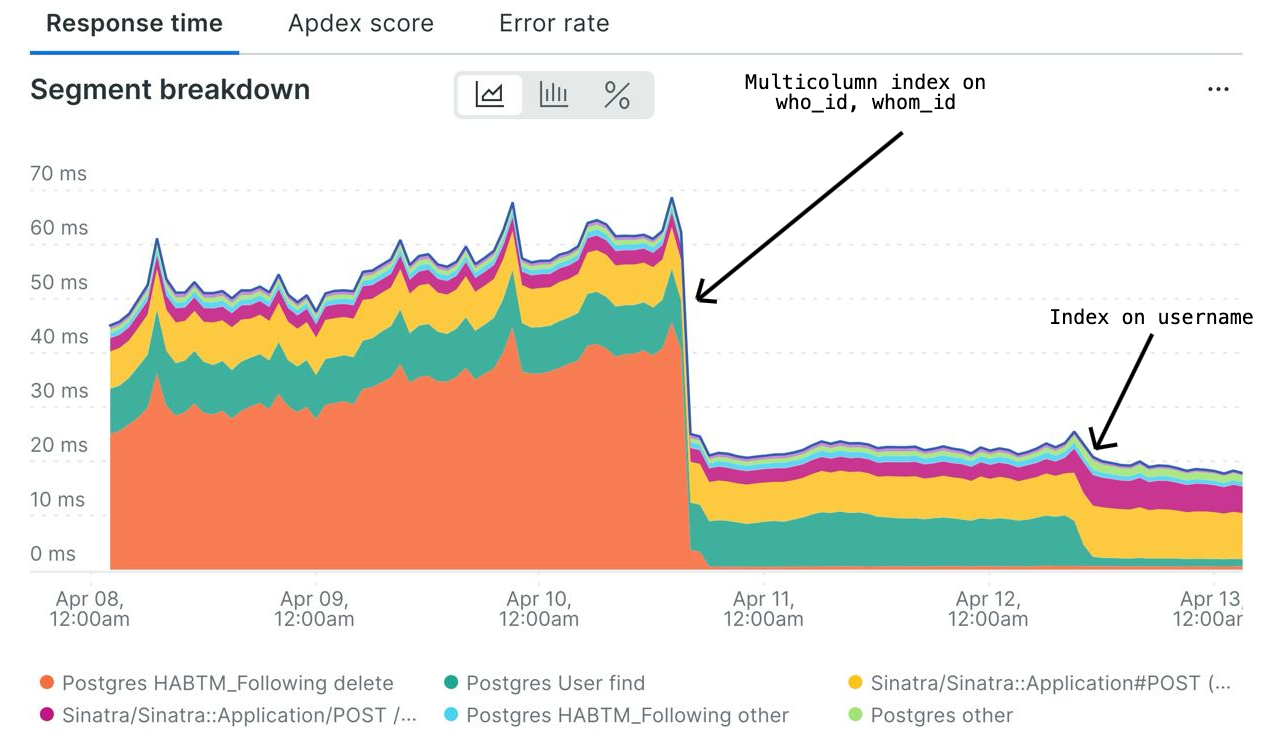
\includegraphics[width=\textwidth]{images/index_apm.png}
    \caption{The APM graph on New Relic, before and after adding indexes}
    \label{fig:index_apm}
\end{figure}
\\Similarly, looking at the graph we saw that a considerable amount of time was spent on the \texttt{GET /user} endpoint. Since users are found by querying by the username, we realized this could be fixed with an index on username. The effect of this can be seen on Figure \ref{fig:index_apm}.
\\\\
When deploying using our deployment pipeline, we would be using some files that are located in \texttt{./remote\_files/}, responsible for pulling the Docker images and starting the Docker swarm. These files are usually uploaded to the manager node using Vagrant or manually \texttt{scp}'ing the files onto the machine. This allows the Github Actions workflow to execute the \texttt{./remote\_files/deploy.sh} script.
However, since we don't often make changes to these files, we would risk forgetting to upload these files when we would actually make changes and there would be room for error causing unwanted or unexpected behaviour.
This caused an issue for us in the same database migration as previously mentioned. This margin for error could be decreased by using a declarative language to configure our infrastructure such as Ansible\footnote{\href{https://www.ansible.com/}{https://www.ansible.com/}} or Terraform\footnote{\href{https://www.terraform.io/}{https://www.terraform.io/}}, or a simpler imperative solution by copying over the files in the deployment workflow. We attempted to implement a Terraform solution, but due to multiple issues we did not get to implement Terraform\footnote{\href{https://github.com/git-gurus-itu-devops/itu-minitwit/pull/75}{https://github.com/git-gurus-itu-devops/itu-minitwit/pull/75}}.

By aborting deployment if testing fails, we allow ourselves to deploy small fixes fast with less uncertainty.
This means we can make quick fixes in order to fix production issues fast and then later address the added technical debt when time allows it.
One example of this is the user validation which was first transferred looking like the old Python code, but later we would implement validation through our ORM-library Active Record for better code quality\footnote{https://github.com/git-gurus-itu-devops/itu-minitwit/pull/43}. 

% This project has differed from others where we were able to make quick fixes that resolves issues present in production quickly and ``fix'' the technical debt at a later stage when the issue is not as urgent. One example of this is the user validation which we would first transfer from the Python codebase to Ruby with a simple helper-function to ensure that a value is neither \texttt{null} or empty when passing it on. However, once we had the time to look further into our ORM-library Active Record, we would rewrite this helper-method to instead use the native validation methods provided by Active Record.
% evt. noget om testing i CI men i am not sure hvilken vinkel



% One of the bigger challenges we faced, was in our attempt to migrate from our manually configured Docker Swarm infrastructure to an Infrastructure-as-Code solution using Terraform. We attempted to create a configuration that spawned our virtual machines on DigitalOcean, and then provision them using inline Bash execution. This was to be part of our CI/CD pipeline, to ensure our infrastructure is able to sync with changes to the configuration automatically.

% However, as Terraform does not handle state of the provisioning, this introduced 

% % We ended up not implenting it fully, as we encountered many complexities regarding the frequency of which the te

% However, we decided against implementing this fully as the complexity level of the configuration grew. Having to provision using Bash scripts proved to be a challenge, as Terraform does not manage the state of these inline provision steps. Any changes to the provisioning steps would then not be synced after creation, which defeats the purpose of having this setup run in the pipeline. Additionally, making sure an SSL-certificate was present each time the infrastructure was created also proved troublesome, as this would either require saving a previously created certificate externally, or running Certbot every time the infrastructure is spawned.

% The provisioning of the infrastructure could have instead been managed by a declarative tool like the previously managed Ansible, as these tools are able to manage the state of provisioning and sync changes. However, as only a single group member had experience using Ansible, we decided against the added complexity of introduction another tool.

% Given these challenges, we decided to stay with our manually configured setup, as we did not feel we had the time to implement the setup in a satisfactory way.




\newpage
\appendix
\section{Appendix}

\subsection{Development dependency graph} \label{appendix: dev-dependecies}
\begin{figure}[H]
    \centering
    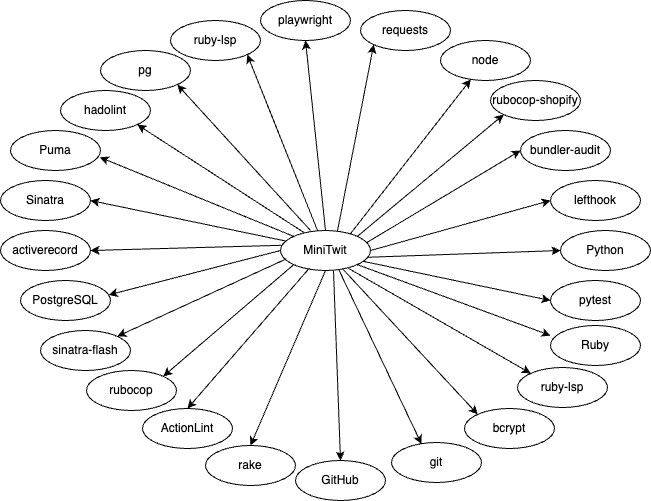
\includegraphics[width=\textwidth]{images/dependency-graph-dev.png}
    \caption{Development dependency graph.}
    \label{fig:dep-dev}
\end{figure}

\end{document}





